\documentclass{beamer}

% to include graphics
\usepackage{graphicx}

% to include hyperlinks
\usepackage{hyperref}

% divide slides into columns
\usepackage{multicol}


\usetheme{Copenhagen}
\usecolortheme{beaver}

\title{Cluster Progress}
\date{\today}

\begin{document}

%----------BEGIN TITLE----------

\begin{frame}
  \maketitle
\end{frame}

%-----------END TITLE-----------

%----------BEGIN NODES----------

\begin{frame}

  \frametitle{Component Incorporation}
  
  \begin{multicols}{2}

    \begin{itemize}
    \item Renaming the Nodes
      \begin{itemize}
      \item The nodes in cabinet 0 have been renamed. They now belong to cabinet 2.
      \end{itemize}
    \item Incorporating the SE
      \begin{itemize}
      \item The SE has been added as {\tt compute-0-10}.
      \end{itemize}
    \end{itemize}
    
    \columnbreak
    
    \begin{figure}[H]
      \begin{center}
        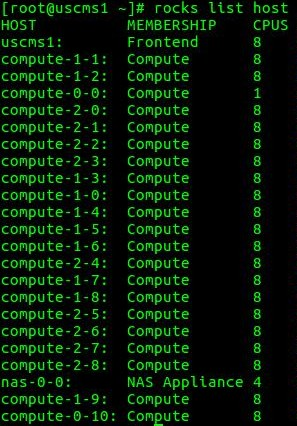
\includegraphics[scale=0.35]{renamed_nodes.png}
      \end{center}
      \caption{The nodes in cabinet ``0'' have been renamed.}
    \end{figure}
  
  \end{multicols}
  
\end{frame}


%-----------END NODES-----------

%----------BEGIN NAS-0----------

\begin{frame}

  \frametitle{NAS-0 Issues}

  \begin{itemize}
    \item The OS RAID array is degraded.
    \item One of the two mirrored drives has failed.
    \item NAS-0 failed to recognize the replacement drive.
    \item Both drives are being tested.
  \end{itemize}

\end{frame}

%-----------END NAS-0-----------



\end{document}

